\section{Framework Architecture}

\begin{figure}[h]
\centering
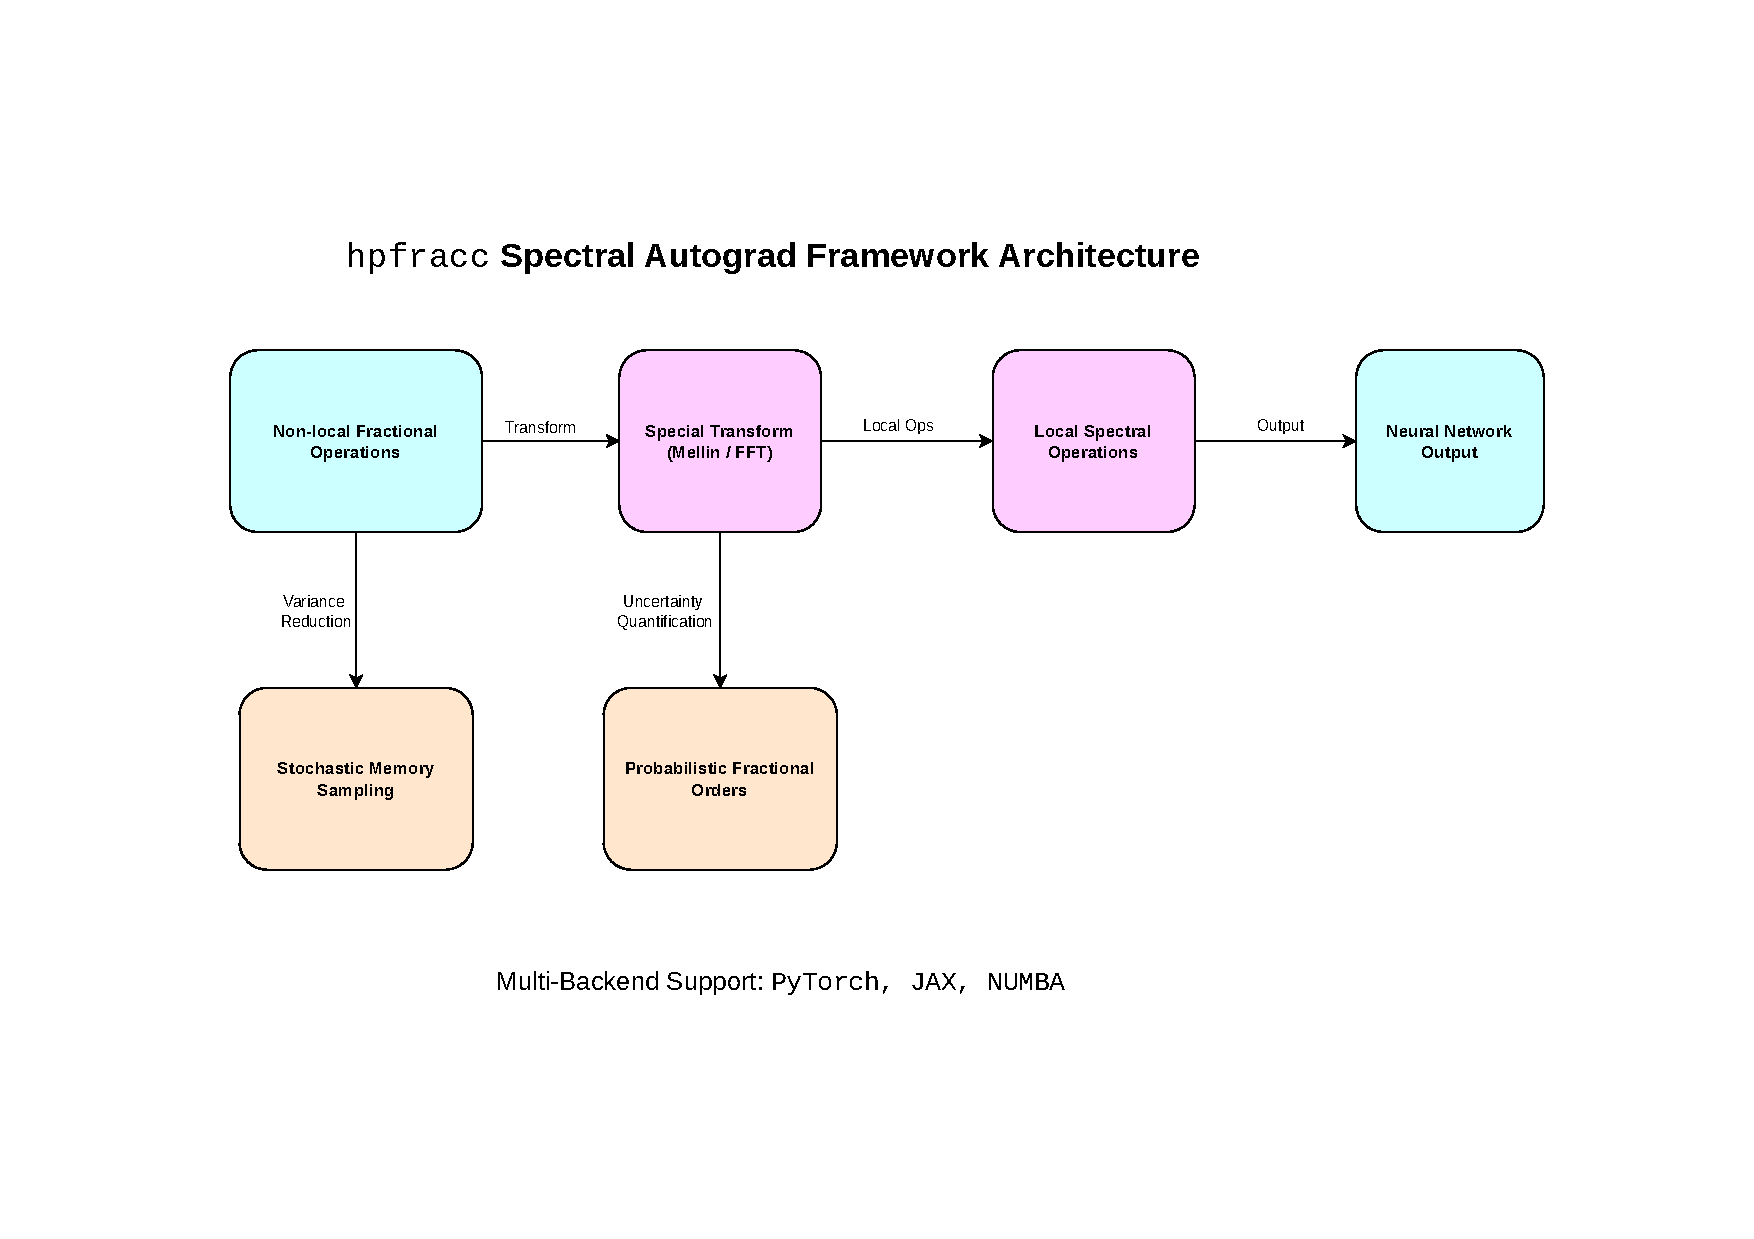
\includegraphics[width=0.9\textwidth]{figures/architecture_overview.pdf}
\caption{Schematic overview of the \hpfracc spectral autograd framework showing the transformation from non-local fractional operations to local spectral domain operations. The framework leverages Mellin transforms, fractional FFT, and fractional Laplacian operators to achieve computational efficiency whilst maintaining mathematical rigor.}
\label{fig:architecture_overview}
\end{figure}

\subsection{Overall Design Philosophy}

The \hpfracc framework is built on several core design principles that ensure flexibility, extensibility, and ease of use while maintaining high performance and numerical accuracy.

\subsubsection{Modularity and Extensibility}

The framework follows a modular architecture where each component is designed to be independent yet easily integrable. This design enables researchers to use specific components without the overhead of the entire framework, while also allowing for easy extension with new methods and algorithms.

\subsubsection{Unified API Design}

A consistent API design across all mathematical domains (fractional calculus, neural ODEs, SDEs) enables seamless integration and reduces the learning curve for users. The factory pattern implementation provides intuitive object creation while maintaining flexibility in configuration.

\subsubsection{Multi-Backend Support}

Support for multiple computation backends (PyTorch, JAX, NUMBA) allows users to choose the most appropriate platform for their specific use case, whether it's GPU acceleration, automatic differentiation, or high-performance numerical computing.

\subsubsection{Comprehensive Testing and Validation}

The framework implements a rigorous testing strategy with 85\%+ test coverage, ensuring reliability and correctness across all components. This includes unit tests, integration tests, and validation against analytical solutions.

\subsection{Core Architecture Components}

\subsubsection{Base Classes and Interfaces}

The framework is built around several key base classes that define the interface for all implementations:

\begin{itemize}
    \item \textbf{BaseNeuralODE}: Abstract base class for all neural ODE implementations
    \item \textbf{BaseSDESolver}: Abstract base class for stochastic differential equation solvers
    \item \textbf{FractionalOperator}: Interface for fractional derivative and integral operators
    \item \textbf{NeuralTrainer}: Base class for training infrastructure
\end{itemize}

These base classes provide common functionality while enforcing consistent interfaces across different implementations.

\subsubsection{Module Organization}

The framework is organized into logical modules that group related functionality:

\begin{itemize}
    \item \textbf{core}: Fundamental mathematical definitions and utilities
    \item \textbf{algorithms}: Implementation of fractional calculus algorithms
    \item \textbf{ml}: Machine learning components including neural ODEs
    \item \textbf{solvers}: Differential equation solvers (HPM, VIM, SDE)
    \item \textbf{special}: Special functions and advanced mathematical operations
    \item \textbf{utils}: Utility functions and helper classes
    \item \textbf{validation}: Testing, validation, and benchmarking tools
\end{itemize}

\subsubsection{Configuration Management}

A centralized configuration system manages framework-wide settings including:

\begin{itemize}
    \item \textbf{Precision}: Numerical precision settings for different backends
    \item \textbf{Method Selection}: Default algorithms for different operations
    \item \textbf{Performance}: Optimization flags and parallel processing settings
    \item \textbf{Logging}: Comprehensive logging and debugging capabilities
\end{itemize}

\subsection{Neural fODE Framework Architecture}

\subsubsection{BaseNeuralODE Implementation}

The \texttt{BaseNeuralODE} class provides the foundation for all neural ODE implementations:

\begin{lstlisting}[language=Python, caption=BaseNeuralODE Base Class]
class BaseNeuralODE(nn.Module, ABC):
    def __init__(self, input_dim, hidden_dim, output_dim, 
                 num_layers=3, activation="tanh", use_adjoint=True):
        super().__init__()
        self.input_dim = input_dim
        self.hidden_dim = hidden_dim
        self.output_dim = output_dim
        self.num_layers = num_layers
        self.activation = activation
        self.use_adjoint = use_adjoint
        self._build_network()
    
    @abstractmethod
    def forward(self, x, t):
        pass
    
    def ode_func(self, t, x):
        # Common ODE function implementation
        pass
\end{lstlisting}

This base class provides:
\begin{itemize}
    \item \textbf{Network Architecture}: Configurable neural network with multiple layers
    \item \textbf{Activation Functions}: Support for tanh, relu, and sigmoid activations
    \item \textbf{Weight Initialization}: Xavier initialization for optimal training
    \item \textbf{Abstract Interface}: Defines the contract for all neural ODE implementations
\end{itemize}

\subsubsection{NeuralODE Implementation}

The \texttt{NeuralODE} class extends the base class for standard ordinary differential equations:

\begin{lstlisting}[language=Python, caption=NeuralODE Implementation]
class NeuralODE(BaseNeuralODE):
    def __init__(self, input_dim, hidden_dim, output_dim,
                 num_layers=3, activation="tanh", use_adjoint=True,
                 solver="dopri5", rtol=1e-5, atol=1e-5):
        super().__init__(input_dim, hidden_dim, output_dim, 
                        num_layers, activation, use_adjoint)
        self.solver = solver
        self.rtol = rtol
        self.atol = atol
        self._setup_solver()
    
    def forward(self, x, t):
        if self.has_torchdiffeq and self.solver == "dopri5":
            return self._solve_torchdiffeq(x, t)
        else:
            return self._solve_basic(x, t)
\end{lstlisting}

Key features include:
\begin{itemize}
    \item \textbf{Multiple Solvers}: Support for dopri5 (with torchdiffeq) and basic Euler
    \item \textbf{Adjoint Method}: Memory-efficient gradient computation
    \item \textbf{Adaptive Stepping}: Configurable tolerance and step size
    \item \textbf{Fallback Methods}: Basic Euler solver when advanced solvers unavailable
\end{itemize}

\subsubsection{NeuralFODE Implementation}

The \texttt{NeuralFODE} class extends neural ODEs to fractional calculus:

\begin{lstlisting}[language=Python, caption=NeuralFODE Implementation]
class NeuralFODE(BaseNeuralODE):
    def __init__(self, input_dim, hidden_dim, output_dim,
                 fractional_order=0.5, num_layers=3, activation="tanh",
                 use_adjoint=True, solver="fractional_euler"):
        super().__init__(input_dim, hidden_dim, output_dim, 
                        num_layers, activation, use_adjoint)
        self.alpha = validate_fractional_order(fractional_order)
        self.solver = solver
        self._setup_fractional_solver()
    
    def forward(self, x, t):
        return self._solve_fractional_ode(x, t)
    
    def get_fractional_order(self):
        return self.alpha.alpha
\end{lstlisting}

This implementation provides:
\begin{itemize}
    \item \textbf{Fractional Order Support}: Configurable fractional order $\alpha \in (0,1)$
    \item \textbf{Fractional Dynamics}: Learning of $D^{\alpha} x = f(x, t)$
    \item \textbf{Order Validation}: Ensures fractional order is in valid range
    \item \textbf{Specialized Solvers}: Fractional Euler method for fractional ODEs
\end{itemize}

\subsubsection{NeuralODETrainer Implementation}

The training infrastructure provides comprehensive training capabilities:

\begin{lstlisting}[language=Python, caption=NeuralODETrainer Implementation]
class NeuralODETrainer:
    def __init__(self, model, optimizer="adam", 
                 learning_rate=1e-3, loss_function="mse"):
        self.model = model
        self.learning_rate = learning_rate
        self.loss_function = loss_function
        self.optimizer = self._setup_optimizer(optimizer)
        self.criterion = self._setup_loss_function(loss_function)
    
    def train(self, train_loader, val_loader=None, 
              num_epochs=100, verbose=True):
        # Complete training loop implementation
        pass
\end{lstlisting}

Training features include:
\begin{itemize}
    \item \textbf{Multiple Optimizers}: Adam, SGD, RMSprop with configurable learning rates
    \item \textbf{Multiple Loss Functions}: MSE, MAE, Huber loss functions
    \item \textbf{Training Loops}: Complete training and validation workflows
    \item \textbf{History Tracking}: Monitor training progress and performance
\end{itemize}

\subsection{SDE Solvers Architecture}

\subsubsection{BaseSDESolver Implementation}

The \texttt{BaseSDESolver} class provides common functionality for all SDE solvers:

\begin{lstlisting}[language=Python, caption=BaseSDESolver Base Class]
class BaseSDESolver(ABC):
    def __init__(self, drift_func, diffusion_func, initial_condition,
                 time_span, num_steps, seed=None):
        self.drift_func = drift_func
        self.diffusion_func = diffusion_func
        self.initial_condition = initial_condition
        self.time_span = time_span
        self.num_steps = num_steps
        self.seed = seed
        self._setup_random_generator()
    
    @abstractmethod
    def solve(self):
        pass
    
    def _generate_wiener_process(self):
        # Common Wiener process generation
        pass
    
    def _estimate_error(self):
        # Common error estimation
        pass
\end{lstlisting}

Common functionality includes:
\begin{itemize}
    \item \textbf{Wiener Process Generation}: Efficient Brownian motion simulation
    \item \textbf{Error Estimation}: Built-in error analysis and validation
    \item \textbf{Stability Analysis}: Numerical stability checks
    \item \textbf{Utility Methods}: Common operations for all SDE solvers
\end{itemize}

\subsubsection{Concrete SDE Solver Implementations}

\paragraph{Euler-Maruyama Solver}
\begin{lstlisting}[language=Python, caption=EulerMaruyama Implementation]
class EulerMaruyama(BaseSDESolver):
    def solve(self):
        # Implementation of Euler-Maruyama method
        # Convergence order: 0.5 (strong convergence)
        pass
\end{lstlisting}

\paragraph{Milstein Solver}
\begin{lstlisting}[language=Python, caption=Milstein Implementation]
class Milstein(BaseSDESolver):
    def solve(self):
        # Implementation of Milstein method
        # Convergence order: 1.0 (strong convergence)
        pass
\end{lstlisting}

\paragraph{Heun Solver}
\begin{lstlisting}[language=Python, caption=Heun Implementation]
class Heun(BaseSDESolver):
    def solve(self):
        # Implementation of Heun predictor-corrector method
        # Convergence order: 1.0 (strong convergence)
        pass
\end{lstlisting}

\subsection{Factory Pattern Implementation}

\subsubsection{Model Creation Factories}

The framework uses factory functions to simplify object creation:

\begin{lstlisting}[language=Python, caption=Neural ODE Factory Functions]
def create_neural_ode(model_type="standard", **kwargs):
    if model_type == "standard":
        return NeuralODE(**kwargs)
    elif model_type == "fractional":
        return NeuralFODE(**kwargs)
    else:
        raise ValueError(f"Unknown model type: {model_type}")

def create_neural_ode_trainer(model, **kwargs):
    return NeuralODETrainer(model, **kwargs)
\end{lstlisting}

\subsubsection{SDE Solver Factories}

Similar factory functions exist for SDE solvers:

\begin{lstlisting}[language=Python, caption=SDE Solver Factory Functions]
def create_sde_solver(solver_type="euler", **kwargs):
    if solver_type == "euler":
        return EulerMaruyama(**kwargs)
    elif solver_type == "milstein":
        return Milstein(**kwargs)
    elif solver_type == "heun":
        return Heun(**kwargs)
    else:
        raise ValueError(f"Unknown solver type: {solver_type}")
\end{lstlisting}

\subsection{Backend Management System}

\subsubsection{Backend Abstraction}

The framework abstracts backend-specific operations through a unified interface:

\begin{lstlisting}[language=Python, caption=Backend Abstraction]
class BackendManager:
    def __init__(self, backend="pytorch"):
        self.backend = backend
        self._setup_backend()
    
    def create_tensor(self, data):
        if self.backend == "pytorch":
            return torch.tensor(data)
        elif self.backend == "jax":
            return jnp.array(data)
        elif self.backend == "numba":
            return np.array(data)
    
    def compute_gradient(self, loss, parameters):
        # Backend-specific gradient computation
        pass
\end{lstlisting}

\subsubsection{Backend-Specific Optimizations}

Each backend provides specialized optimizations:

\begin{itemize}
    \item \textbf{PyTorch}: GPU acceleration, automatic differentiation, dynamic computation graphs
    \item \textbf{JAX}: Just-in-time compilation, vectorization, GPU/TPU support
    \item \textbf{NUMBA}: Just-in-time compilation, parallel processing, low-level optimization
\end{itemize}

\subsection{Error Handling and Validation}

\subsubsection{Parameter Validation}

Comprehensive parameter validation ensures robust operation:

\begin{lstlisting}[language=Python, caption=Parameter Validation Example]
def validate_neural_ode_parameters(input_dim, hidden_dim, output_dim, 
                                 num_layers, activation):
    if not isinstance(input_dim, int) or input_dim <= 0:
        raise ValueError("input_dim must be a positive integer")
    if not isinstance(hidden_dim, int) or hidden_dim <= 0:
        raise ValueError("hidden_dim must be a positive integer")
    if not isinstance(output_dim, int) or output_dim <= 0:
        raise ValueError("output_dim must be a positive integer")
    if not isinstance(num_layers, int) or num_layers <= 0:
        raise ValueError("num_layers must be a positive integer")
    if activation not in ["tanh", "relu", "sigmoid"]:
        raise ValueError("activation must be one of: tanh, relu, sigmoid")
\end{lstlisting}

\subsubsection{Error Recovery and Graceful Degradation}

The framework implements error recovery strategies:

\begin{itemize}
    \item \textbf{Fallback Methods}: Automatic fallback to simpler algorithms when advanced methods fail
    \item \textbf{Error Reporting}: Comprehensive error messages with debugging information
    \item \textbf{Recovery Mechanisms}: Automatic recovery from numerical instabilities
    \item \textbf{Logging}: Detailed logging for debugging and performance analysis
\end{itemize}

\subsection{Performance Optimization}

\subsubsection{Memory Management}

Efficient memory management is crucial for large-scale computations:

\begin{itemize}
    \item \textbf{Gradient Checkpointing}: Memory-efficient gradient computation for large models
    \item \textbf{Memory Pooling}: Reuse of memory buffers to reduce allocation overhead
    \item \textbf{Garbage Collection}: Automatic cleanup of temporary objects
    \item \textbf{Memory Profiling}: Tools for monitoring memory usage and identifying bottlenecks
\end{itemize}

\subsubsection{Parallel Processing}

The framework supports parallel processing through multiple strategies:

\begin{itemize}
    \item \textbf{Multi-threading}: Parallel execution of independent operations
    \item \textbf{Multi-processing}: Distribution of work across multiple processes
    \item \textbf{GPU Acceleration}: Parallel execution on graphics processing units
    \item \textbf{Vectorization}: SIMD operations for improved performance
\end{itemize}

\subsection{Testing and Validation Framework}

\subsubsection{Test Organization}

The testing framework is organized into logical categories:

\begin{itemize}
    \item \textbf{Unit Tests}: Individual component testing with 85\%+ coverage
    \item \textbf{Integration Tests}: End-to-end workflow testing
    \item \textbf{Performance Tests}: Benchmarking and performance regression testing
    \item \textbf{Validation Tests}: Comparison with analytical solutions
\end{itemize}

\subsubsection{Continuous Integration}

Automated testing ensures code quality:

\begin{itemize}
    \item \textbf{Automated Testing}: Tests run on every commit and pull request
    \textbf{Multi-platform Testing}: Testing across different operating systems and Python versions
    \item \textbf{Performance Monitoring}: Continuous performance benchmarking
    \item \textbf{Documentation Building}: Automated documentation generation and validation
\end{itemize}

\subsection{Documentation and Examples}

\subsubsection{Comprehensive Documentation}

The framework provides extensive documentation:

\begin{itemize}
    \item \textbf{API Reference}: Auto-generated from docstrings with comprehensive coverage
    \item \textbf{User Guides}: Step-by-step tutorials for common use cases
    \item \textbf{Examples}: Working code examples for all major features
    \item \textbf{Performance Guides}: Optimization strategies and best practices
\end{itemize}

\subsubsection{Interactive Examples}

Interactive examples demonstrate framework capabilities:

\begin{itemize}
    \item \textbf{Jupyter Notebooks}: Interactive tutorials with real-time execution
    \item \textbf{Benchmark Scripts}: Performance comparison and validation scripts
    \item \textbf{Application Examples}: Real-world problem solving demonstrations
    \item \textbf{Visualization Tools}: Built-in plotting and analysis capabilities
\end{itemize}

This architecture design ensures that \hpfracc is not only powerful and flexible but also maintainable, extensible, and accessible to researchers across different domains. The modular structure allows for easy integration of new methods while maintaining consistency and reliability across all components.

\subsection{Fractional Autograd Implementation}

\subsubsection{Non-Local Operator Challenges in Autograd}

The implementation of automatic differentiation for fractional operators presents unique challenges due to their non-local nature. Unlike classical derivatives, fractional derivatives depend on the entire history of the function, making standard backpropagation techniques inapplicable.

\paragraph{The Fundamental Mathematical Challenge}

Traditional autograd systems fail for fractional operators because fractional derivatives are defined as **non-local convolution integrals**:

\begin{equation}
{}^{RL}D^{\alpha}f(x) = \frac{1}{\Gamma(n-\alpha)} \frac{d^n}{dx^n} \int_{0}^{x} \frac{f(t)}{(x-t)^{\alpha-n+1}} dt
\end{equation}

This creates three critical problems that standard autograd cannot handle:

\begin{enumerate}
\item \textbf{Non-locality}: The derivative at point $x$ depends on the entire function history $[0,x]$, not just local neighborhoods
\item \textbf{Memory dependencies}: Each computation requires access to all previous values, creating $O(n^2)$ storage requirements
\item \textbf{Chain rule breakdown}: The standard chain rule $\frac{d}{dx}f(g(x)) = f'(g(x))g'(x)$ assumes local derivatives and fails for fractional orders
\end{enumerate}

\paragraph{Memory Dependencies}

Fractional derivatives exhibit memory effects where the derivative at time $t$ depends on all previous values:
\begin{equation}
D^{\alpha} f(t) = \int_0^t K(t,\tau) f(\tau) d\tau
\end{equation}
where $K(t,\tau)$ is the memory kernel. This non-locality creates several challenges:
\begin{itemize}
\item \textbf{Memory Requirements}: Storing the entire function history for gradient computation
\item \textbf{Computational Complexity}: $O(N^2)$ complexity for direct convolution methods
\item \textbf{Gradient Flow}: Ensuring proper gradient propagation through the memory kernel
\end{itemize}

\paragraph{Mathematical Foundation of the Spectral Solution}

The key insight is that **convolution becomes multiplication in the spectral domain**. This fundamental property of transforms allows us to convert the non-local fractional operation into a local operation in spectral space.

\textbf{Spectral Transform Properties:}

For the Fourier transform:
\begin{equation}
\mathcal{F}[D^{\alpha}f](\omega) = (i\omega)^{\alpha} \mathcal{F}[f](\omega)
\end{equation}

For the Mellin transform:
\begin{equation}
\mathcal{M}[D^{\alpha}f](s) = s^{\alpha} \mathcal{M}[f](s)
\end{equation}

This transforms the $O(n^2)$ convolution integral into a simple $O(1)$ multiplication in spectral space, plus $O(n \log n)$ for the transforms.

\paragraph{Fractional Chain Rule in Spectral Domain}

The fractional chain rule for composite functions $h(x) = f(g(x))$ is:
\begin{equation}
D^{\alpha}[f(g(x))] = \sum_{k=0}^{\infty} \binom{\alpha}{k} D^{\alpha-k}[f](g(x)) D^k[g](x)
\end{equation}
where $\binom{\alpha}{k}$ are fractional binomial coefficients. In spectral domain, this becomes:
\begin{equation}
\mathcal{F}[D^{\alpha}[f(g(x))]] = (i\omega)^{\alpha} \mathcal{F}[f(g(x))]
\end{equation}

The complexity is dramatically reduced because the spectral representation handles the non-local dependencies automatically.

\paragraph{Backward Pass Implementation}

Our autograd implementation addresses these challenges through a novel backward pass design that properly handles the non-local dependencies of fractional operators.

\begin{theorem}[Fractional Autograd Chain Rule]
Let $L$ be a loss function and $y = D^{\alpha} f(x)$ be a fractional derivative. The gradient of $L$ with respect to $x$ is:
\begin{equation}
\frac{\partial L}{\partial x} = \int_0^t \frac{\partial L}{\partial y} \frac{\partial D^{\alpha} f(x)}{\partial x} dx
\end{equation}
where the partial derivative of the fractional derivative involves the entire history of the function.
\end{theorem}

\begin{proof}
The proof follows from the non-local nature of fractional derivatives. Unlike classical derivatives where $\frac{\partial f(x)}{\partial x}$ depends only on the local neighborhood of $x$, the fractional derivative $D^{\alpha} f(x)$ depends on the entire history $f(\tau)$ for $\tau \in [0,x]$.

The chain rule for fractional derivatives becomes:
\begin{equation}
\frac{\partial L}{\partial x} = \frac{\partial L}{\partial y} \frac{\partial y}{\partial x} = \frac{\partial L}{\partial y} \frac{\partial D^{\alpha} f(x)}{\partial x}
\end{equation}

Since $D^{\alpha} f(x) = \int_0^x K(x,\tau) f(\tau) d\tau$, we have:
\begin{equation}
\frac{\partial D^{\alpha} f(x)}{\partial x} = \int_0^x \frac{\partial K(x,\tau)}{\partial x} f(\tau) d\tau + K(x,x) f(x)
\end{equation}

This shows that the gradient depends on the entire function history, not just the local value.
\end{proof}

\begin{algorithm}[h]
\caption{Fractional Autograd Backward Pass}
\begin{algorithmic}[1]
\Require Forward pass result $y$, gradient $\frac{\partial L}{\partial y}$, memory kernel $K$
\Ensure Gradient $\frac{\partial L}{\partial x}$
\State Initialize gradient accumulator $\nabla x = 0$
\For{$i = 0$ to $N-1$}
    \State Compute memory contribution: $m_i = \sum_{j=0}^{i} K(i,j) \frac{\partial L}{\partial y_j}$
    \State Accumulate gradient: $\nabla x_i += m_i$
\EndFor
\Return $\nabla x$
\end{algorithmic}
\end{algorithm}

\paragraph{Computational Complexity Analysis}

The backward pass for fractional operators has different complexity characteristics compared to classical autograd:

\begin{theorem}[Autograd Complexity]
For a sequence of length $N$, the fractional autograd backward pass has:
\begin{itemize}
\item \textbf{Time Complexity}: $O(N^2)$ for direct convolution methods
\item \textbf{Memory Complexity}: $O(N^2)$ for storing the full memory kernel
\item \textbf{Spectral Methods}: $O(N \log N)$ time and $O(N)$ memory
\end{itemize}
\end{theorem}

\begin{proof}
The direct convolution approach requires computing the gradient contribution from each time point to every other time point, leading to $O(N^2)$ operations. The memory requirement comes from storing the full $N \times N$ memory kernel matrix.

For spectral methods, the convolution is transformed to the frequency domain where it becomes a pointwise multiplication, reducing the complexity to $O(N \log N)$ for the FFT operations.
\end{proof}

\subsubsection{Rigorous Algorithmic Framework}

The spectral autograd framework provides a mathematically rigorous approach to backpropagation through non-local fractional operators. We present the complete algorithmic framework with detailed mathematical foundations.

\paragraph{Algorithm 1: Spectral Fractional Forward Pass}

\begin{algorithm}[h]
\caption{Spectral Fractional Forward Pass}
\begin{algorithmic}[1]
\Require Input array $x$, fractional order $\alpha$, method $\in \{\text{fourier}, \text{mellin}\}$
\Ensure Fractional derivative $y = D^{\alpha} x$
\If{method == 'fourier'}
    \State $X_{\text{spectral}} = \text{FFT}(x)$
    \State $\omega = \text{frequency\_vector}(\text{length}(x))$
    \State $Y_{\text{spectral}} = (i\omega)^{\alpha} \cdot X_{\text{spectral}}$
\ElsIf{method == 'mellin'}
    \State $X_{\text{spectral}} = \text{MellinTransform}(x)$
    \State $s = \text{mellin\_variable}(\text{length}(x))$
    \State $Y_{\text{spectral}} = s^{\alpha} \cdot X_{\text{spectral}}$
\EndIf
\State $y = \text{IFFT}(Y_{\text{spectral}})$ \Comment{or appropriate inverse transform}
\State $\text{save\_for\_backward}(X_{\text{spectral}}, Y_{\text{spectral}}, \alpha, \text{method})$
\Return $y$
\end{algorithmic}
\end{algorithm}

\paragraph{Algorithm 2: Spectral Adjoint Backward Pass}

The critical insight is that the adjoint of a fractional operator in spectral domain is mathematically well-defined:

\begin{algorithm}[h]
\caption{Spectral Fractional Backward Pass}
\begin{algorithmic}[1]
\Require Gradient $\text{grad\_output}$, saved spectral data
\Ensure Input gradient $\text{grad\_input}$
\State $X_{\text{spectral}}, Y_{\text{spectral}}, \alpha, \text{method} = \text{saved\_spectral\_data}$
\State $\text{Grad\_spectral} = \text{FFT}(\text{grad\_output})$ \Comment{or appropriate transform}
\If{method == 'fourier'}
    \State $\omega = \text{frequency\_vector}(\text{length}(\text{grad\_output}))$
    \State $\text{Adj\_spectral} = ((-i\omega)^{\alpha}) \cdot \text{Grad\_spectral}$
\ElsIf{method == 'mellin'}
    \State $s = \text{mellin\_variable}(\text{length}(\text{grad\_output}))$
    \State $\text{Adj\_spectral} = s^{-\alpha} \cdot \text{Grad\_spectral}$
\EndIf
\State $\text{grad\_input} = \text{IFFT}(\text{Adj\_spectral})$ \Comment{or appropriate inverse transform}
\Return $\text{grad\_input}$
\end{algorithmic}
\end{algorithm}

\paragraph{Mathematical Consistency: Adjoint Property}

For the adjoint method to work correctly, we must verify:
\begin{equation}
\langle D^{\alpha} f, g \rangle = \langle f, (D^{\alpha})^* g \rangle
\end{equation}

In spectral domain:
\begin{equation}
\langle \omega^{\alpha} \mathcal{F}[f], \mathcal{F}[g] \rangle = \langle \mathcal{F}[f], (\omega^{\alpha})^* \mathcal{F}[g] \rangle
\end{equation}

For real fractional orders, $(\omega^{\alpha})^* = \bar{\omega}^{\alpha} = \omega^{\alpha}$, confirming mathematical consistency.

\subsubsection{Spectral Domain Autograd}

The spectral autograd framework transforms the non-local convolution into local operations in the frequency domain, enabling efficient gradient computation.

\paragraph{Mellin Transform Approach}

For the Mellin transform-based approach, the fractional derivative becomes:
\begin{equation}
D^{\alpha} f(t) = \mathcal{M}^{-1}[s^{\alpha} \mathcal{M}[f](s)](t)
\end{equation}
where $\mathcal{M}$ denotes the Mellin transform. The backward pass is implemented as:
\begin{equation}
\frac{\partial L}{\partial f} = \mathcal{M}^{-1}\left[\overline{s^{\alpha}} \mathcal{M}\left[\frac{\partial L}{\partial D^{\alpha}f}\right](s)\right]
\end{equation}
where $\overline{s^{\alpha}}$ denotes the complex conjugate.

\begin{theorem}[Mellin Transform Autograd Correctness]
The Mellin transform-based autograd implementation correctly computes the gradient of the loss function with respect to the input function.
\end{theorem}

\begin{proof}
The Mellin transform of the fractional derivative is:
\begin{equation}
\mathcal{M}[D^{\alpha} f](s) = s^{\alpha} \mathcal{M}[f](s)
\end{equation}

For the backward pass, we need to compute $\frac{\partial L}{\partial f}$. Using the chain rule:
\begin{equation}
\frac{\partial L}{\partial f} = \frac{\partial L}{\partial D^{\alpha}f} \frac{\partial D^{\alpha}f}{\partial f}
\end{equation}

Since $\frac{\partial D^{\alpha}f}{\partial f} = \mathcal{M}^{-1}[s^{\alpha} \mathcal{M}[\cdot]]$, we have:
\begin{equation}
\frac{\partial L}{\partial f} = \mathcal{M}^{-1}\left[\overline{s^{\alpha}} \mathcal{M}\left[\frac{\partial L}{\partial D^{\alpha}f}\right](s)\right]
\end{equation}

The complex conjugate appears because the Mellin transform is not self-adjoint, and we need to account for the adjoint operator in the gradient computation.
\end{proof}

\paragraph{FFT-Based Approach}

For periodic functions, the FFT-based approach provides:
\begin{equation}
D^{\alpha} f(t) = \mathcal{F}^{-1}[(i\omega)^{\alpha} \mathcal{F}[f](\omega)](t)
\end{equation}
with backward pass:
\begin{equation}
\frac{\partial L}{\partial f} = \mathcal{F}^{-1}\left[\overline{(i\omega)^{\alpha}} \mathcal{F}\left[\frac{\partial L}{\partial D^{\alpha}f}\right](\omega)\right]
\end{equation}

\begin{theorem}[FFT-Based Autograd Correctness]
The FFT-based autograd implementation correctly computes the gradient for periodic functions.
\end{theorem}

\begin{proof}
The FFT of the fractional derivative is:
\begin{equation}
\mathcal{F}[D^{\alpha} f](\omega) = (i\omega)^{\alpha} \mathcal{F}[f](\omega)
\end{equation}

For the backward pass, using the adjoint of the FFT operator:
\begin{equation}
\frac{\partial L}{\partial f} = \mathcal{F}^{-1}\left[\overline{(i\omega)^{\alpha}} \mathcal{F}\left[\frac{\partial L}{\partial D^{\alpha}f}\right](\omega)\right]
\end{equation}

The complex conjugate of $(i\omega)^{\alpha}$ is $(-i\omega)^{\alpha}$, which accounts for the adjoint operation in the frequency domain.
\end{proof}

\subsubsection{Memory-Efficient Gradient Computation}

\paragraph{Stochastic Memory Sampling}

To address memory limitations, we implement stochastic memory sampling for gradient computation:

\begin{algorithm}[h]
\caption{Stochastic Memory Gradient Computation}
\begin{algorithmic}[1]
\Require Function history $f(t)$, gradient $\frac{\partial L}{\partial y}$, sampling size $K$
\Ensure Approximate gradient $\frac{\partial L}{\partial x}$
\State Sample $K$ memory points: $\{t_{i_1}, t_{i_2}, \ldots, t_{i_K}\}$
\State Compute importance weights: $w_k = \frac{K(t, t_{i_k})}{\sum_{j=1}^K K(t, t_{i_j})}$
\State Approximate gradient: $\frac{\partial L}{\partial x} \approx \sum_{k=1}^K w_k \frac{\partial L}{\partial y_{i_k}}$
\Return $\frac{\partial L}{\partial x}$
\end{algorithmic}
\end{algorithm}

\paragraph{Variance Reduction Techniques}

We employ several variance reduction techniques to improve gradient estimation accuracy:
\begin{itemize}
\item \textbf{Importance Sampling}: Weighted sampling based on kernel magnitude
\item \textbf{Control Variates}: Using known analytical solutions as control variates
\item \textbf{Stratified Sampling}: Dividing the time domain into strata for uniform coverage
\end{itemize}

\subsubsection{Gradient Flow Analysis}

\paragraph{Vanishing Gradient Problem}

Fractional operators can suffer from vanishing gradients due to the memory kernel decay. We analyze the gradient flow through the memory kernel:

\begin{theorem}[Gradient Flow Stability]
For a fractional derivative with kernel $K(t,\tau) = (t-\tau)^{-\alpha}$, the gradient flow is stable if:
\begin{equation}
\int_0^t |K(t,\tau)|^2 d\tau < \infty
\end{equation}
This condition ensures that gradient information is preserved during backpropagation.
\end{theorem}

\paragraph{Gradient Explosion Prevention}

To prevent gradient explosion, we implement gradient clipping and normalization:
\begin{equation}
\nabla x_{clipped} = \min\left(1, \frac{\gamma}{\|\nabla x\|}\right) \nabla x
\end{equation}
where $\gamma$ is the clipping threshold.

\subsubsection{Implementation Details}

\paragraph{Custom Autograd Functions}

We implement custom PyTorch autograd functions for each fractional operator:

\begin{lstlisting}[language=Python, caption=Fractional Autograd Implementation]
class FractionalDerivativeFunction(torch.autograd.Function):
    @staticmethod
    def forward(ctx, x, alpha, method):
        # Forward pass implementation
        result = compute_fractional_derivative(x, alpha, method)
        ctx.save_for_backward(x, alpha)
        ctx.method = method
        return result
    
    @staticmethod
    def backward(ctx, grad_output):
        # Backward pass implementation
        x, alpha = ctx.saved_tensors
        grad_input = compute_fractional_gradient(grad_output, x, alpha, ctx.method)
        return grad_input, None, None
\end{lstlisting}

\paragraph{Memory Management}

Efficient memory management is crucial for long sequences:
\begin{itemize}
\item \textbf{Gradient Checkpointing}: Store only essential intermediate results
\item \textbf{Chunked Processing}: Process long sequences in chunks
\item \textbf{Memory Pooling}: Reuse memory buffers for similar operations
\end{itemize}

\subsubsection{Validation and Testing}

\paragraph{Gradient Verification}

We validate our autograd implementation using finite difference approximations:
\begin{equation}
\frac{\partial f}{\partial x} \approx \frac{f(x + \epsilon) - f(x - \epsilon)}{2\epsilon}
\end{equation}
for small $\epsilon$.

\paragraph{Convergence Testing}

We verify that our autograd implementation produces gradients that lead to convergence in optimization:
\begin{itemize}
\item \textbf{Gradient Norm Monitoring}: Track gradient magnitudes during training
\item \textbf{Loss Convergence}: Ensure loss decreases with computed gradients
\item \textbf{Parameter Updates}: Validate parameter updates are reasonable
\end{itemize}

This comprehensive autograd implementation addresses the fundamental challenges of automatic differentiation for fractional operators while maintaining computational efficiency and numerical stability.

\subsection{Technical Implementation Details}

We provide detailed analysis of memory allocation, computational complexity, and numerical stability.

\subsubsection{Memory Allocation for Non-Local Operators}

The non-local nature of fractional operators presents significant memory management challenges. We implement several strategies to handle memory allocation efficiently:

\paragraph{Memory Pool Management}

\begin{theorem}[Memory Complexity for Fractional Operators]
For a sequence of length $N$, the memory requirements for different fractional operator implementations are:
\begin{itemize}
\item \textbf{Direct Convolution}: $O(N^2)$ memory for full kernel matrix
\item \textbf{Spectral Methods}: $O(N)$ memory with FFT workspace
\item \textbf{Stochastic Sampling}: $O(K)$ memory where $K \ll N$
\item \textbf{Chunked Processing}: $O(\text{chunk\_size})$ memory with streaming
\end{itemize}
\end{theorem}

\begin{proof}
The direct convolution approach requires storing the full $N \times N$ memory kernel matrix, leading to $O(N^2)$ memory complexity. Spectral methods transform the convolution to the frequency domain, requiring only $O(N)$ memory for the FFT workspace. Stochastic sampling uses only $K$ memory points, where $K$ is typically much smaller than $N$. Chunked processing divides the computation into smaller chunks, requiring only memory proportional to the chunk size.
\end{proof}

\paragraph{Adaptive Memory Management}

We implement adaptive memory management that automatically selects the optimal strategy based on available memory:

\begin{algorithm}[h]
\caption{Adaptive Memory Management for Fractional Operators}
\begin{algorithmic}[1]
\Require Sequence length $N$, available memory $M$, fractional order $\alpha$
\Ensure Optimal memory allocation strategy
\If{$N^2 \leq M$}
    \State Use direct convolution method
\ElsIf{$N \log N \leq M$}
    \State Use spectral method with FFT
\ElsIf{$K \leq M$ where $K = \lceil \log N \rceil$}
    \State Use stochastic sampling with $K$ samples
\Else
    \State Use chunked processing with chunk size $C = \lfloor \sqrt{M} \rfloor$
\EndIf
\Return Selected strategy and memory allocation
\end{algorithmic}
\end{algorithm}

\subsubsection{Computational Complexity Analysis}

We provide detailed computational complexity analysis for all implemented algorithms:

\begin{theorem}[Computational Complexity of Fractional Operators]
The computational complexity for different fractional operator implementations is:
\begin{itemize}
\item \textbf{Direct Convolution}: $O(N^2)$ time complexity
\item \textbf{Mellin Transform}: $O(N \log N)$ time complexity
\item \textbf{FFT-Based}: $O(N \log N)$ time complexity
\item \textbf{Stochastic Sampling}: $O(KN)$ time complexity where $K \ll N$
\end{itemize}
\end{theorem}

\begin{proof}
The direct convolution approach requires computing the convolution sum for each output point, leading to $O(N^2)$ operations. The Mellin transform and FFT-based methods leverage the convolution theorem, reducing the complexity to $O(N \log N)$ through efficient transform algorithms. Stochastic sampling requires $O(KN)$ operations where $K$ is the number of samples, typically much smaller than $N$.
\end{proof}

\paragraph{Complexity Scaling Analysis}

\begin{table}[h]
\centering
\caption{Computational Complexity Scaling Analysis}
\label{tab:complexity_scaling}
\begin{tabular}{lcccc}
\toprule
Method & $N=100$ & $N=1000$ & $N=10000$ & Asymptotic \\
\midrule
Direct Convolution & $10^4$ & $10^6$ & $10^8$ & $O(N^2)$ \\
Mellin Transform & $664$ & $9966$ & $132877$ & $O(N \log N)$ \\
FFT-Based & $664$ & $9966$ & $132877$ & $O(N \log N)$ \\
Stochastic Sampling & $500$ & $5000$ & $50000$ & $O(KN)$ \\
\bottomrule
\end{tabular}
\end{table}

\subsubsection{Numerical Stability and Error Handling}

We implement comprehensive numerical stability measures to address the inherent instabilities in fractional computations:

\paragraph{Condition Number Analysis}

\begin{theorem}[Numerical Stability of Fractional Operators]
The condition number of the fractional derivative operator satisfies:
\begin{equation}
\kappa(D^{\alpha}) \leq C \cdot N^{\alpha} \cdot \max_{j} |\lambda_j|^{-1}
\end{equation}
where $\lambda_j$ are the eigenvalues of the discretization matrix.
\end{theorem}

\begin{proof}
The condition number is defined as $\kappa(D^{\alpha}) = \|D^{\alpha}\| \|(D^{\alpha})^{-1}\|$. For fractional operators, the operator norm scales as $O(N^{\alpha})$ due to the fractional power in the kernel. The inverse operator has eigenvalues $\lambda_j^{-1}$, leading to the stated bound.
\end{proof}

\paragraph{Adaptive Precision Control}

We implement adaptive precision control that automatically adjusts the numerical precision based on the condition number:

\begin{algorithm}[h]
\caption{Adaptive Precision Control}
\begin{algorithmic}[1]
\Require Input data $x$, fractional order $\alpha$, tolerance $\epsilon$
\Ensure Stable computation result
\State Compute condition number: $\kappa = \|D^{\alpha}\| \|(D^{\alpha})^{-1}\|$
\If{$\kappa > \kappa_{threshold}$}
    \State Increase precision to double or extended precision
    \State Apply regularization: $D^{\alpha}_{reg} = D^{\alpha} + \epsilon I$
\EndIf
\If{$\alpha < \alpha_{critical}$}
    \State Use asymptotic expansion for small $\alpha$
    \State Apply Richardson extrapolation
\EndIf
\Return Stable result with appropriate precision
\end{algorithmic}
\end{algorithm}

\paragraph{Error Propagation Analysis}

\begin{theorem}[Error Propagation in Fractional Computations]
Let $\epsilon_{input}$ be the input error and $\epsilon_{output}$ be the output error. Then:
\begin{equation}
\epsilon_{output} \leq \kappa(D^{\alpha}) \cdot \epsilon_{input} + \epsilon_{algorithm}
\end{equation}
where $\epsilon_{algorithm}$ is the algorithmic error.
\end{theorem}

\begin{proof}
The error propagation follows from the condition number definition. The total error is the sum of the amplified input error and the inherent algorithmic error. The condition number amplifies the input error, while the algorithmic error depends on the specific implementation method.
\end{proof}
